\documentclass{standalone}

\usepackage{circuitikz}

\begin{document}

% INT_AY22_L25_Fig01_EFD.png

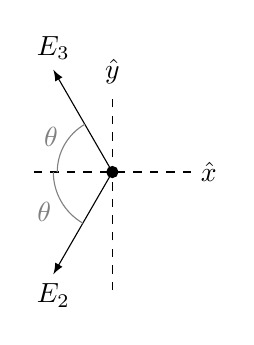
\begin{tikzpicture}[> = latex]

	% Define angle
	
	\def\Q{60}
	
	% The dot
	
	\filldraw (0, 0) circle (2 pt);
	
	% Coordinate axes
	
	\draw [dashed] (-1, 0) -- (1, 0) node [right] {${\hat x}$};
	\draw [dashed] (0, -1.5) -- (0, 1) node [above] {${\hat y}$};
	
	% Forces
	
	\draw [->] (0, 0) -- ({180 + \Q} : 1.5) node [below] {$E_2$};
	\draw [->] (0, 0) -- ({180 - \Q} : 1.5) node [above] {$E_3$};
	
	% Angle indicators
	
	\draw [gray] (-0.7, 0) arc (180 : {180 - \Q} : 0.7);
	\node [gray] at ({180 - 0.5 * \Q} : 0.9) {$\theta$};
	
	\draw [gray] (-0.75, 0) arc (180 : {180 + \Q} : 0.75);
	\node [gray] at ({180 + 0.5 * \Q} : 1) {$\theta$};

\end{tikzpicture}

\end{document}